%!TEX TS-program = xelatex
%!TEX encoding = UTF-8 Unicode

\documentclass[12pt]{article}
\usepackage{geometry}                % See geometry.pdf to learn the layout options. There are lots.
\geometry{a4paper,top=2cm}
\usepackage[parfill]{parskip}    % Activate to begin paragraphs with an empty line rather than an indent
\usepackage{graphicx}
\usepackage{amsmath}
\usepackage{amssymb}
\usepackage{mathtools}
\usepackage{physics}
\newcommand{\be}{\begin{equation}}
\newcommand{\ee}{\end{equation}}
\usepackage[thicklines]{cancel}
\usepackage{url}
\usepackage{booktabs}
\usepackage{qcircuit}
\usepackage{circledsteps}
\usepackage{nicefrac}
\usepackage{fontspec,xltxtra,xunicode}
\defaultfontfeatures{Mapping=tex-text}

\newcommand{\polv}{\ensuremath{\updownarrow}}
\newcommand{\polh}{\ensuremath{\leftrightarrow}}
\newcommand{\poldr}{\rotatebox[origin=c]{45}{\ensuremath{\leftrightarrow}}}
\newcommand{\poldl}{\rotatebox[origin=c]{-45}{\ensuremath{\leftrightarrow}}}

\title{Advanced Quantum Mechanics\\Class 18 (b)}
%\author{The Author}
\date{October 11, 2022}                                           % Activate to display a given date or no date

\setcounter{section}{6}
\setcounter{subsection}{4}
\setcounter{subsubsection}{3}
\setcounter{equation}{81}

\begin{document}
\maketitle

%%% 11 OKAY
\subsection{Conservation laws (continued)}

\subsubsection{Rotation matrices in Hilbert Space (continued)}
 
Under $R$, $\ket{jm}$ transforms to $\ket{jm}_R$ as
\be
\begin{aligned}
\ket{jm}_{R} 
&=\hat{U}[R]\ket{jm}
\sum_{m^{\prime}} \op{jm^\prime} \hat{U}[R] \ket{jm}\\
&=\sum_{m^{\prime}} D^{(j)}_{m^\prime m}[R] \ket{jm^\prime}
\end{aligned}
\ee
From the group composition law (will be shown shortly ahead):
\be
\hat{U}[R_2]\hat{U}[R_1] =
\begin{cases}
+\hat{U}[R_2R_1]&\text{,if $j$ integer}\\
-\hat{U}[R_2R_1]&\text{,if $j$ half-integer}
\end{cases}
\ee
in the basis $\ket{jm}$ this is given by
\be
\begin{gathered}
\bra{jm^\prime}\hat{U}[R_2]
\sum_{m^{\prime\prime}}\op{jm^{\prime\prime}}
\hat{U}[R_1]\ket{jm}=\\
\sum_{m^{\prime\prime}} 
D^{(j)}_{m^\prime m^{\prime\prime}}[R_2]
D^{(j)}_{m^{\prime\prime m}}[R_1] =
\pm D^{(j)}_{m^\prime m}[R_2R_1]
\end{gathered}
\ee

Let us consider now the matrices \(D^{(j)}[R]\) for a generic \(R\).
In principle, one needs three parameters to characterize \(R\):
- usually they are taken to  be the Euler angles \(\alpha, \beta, \gamma\)
%%% 12 OKAY
(see \textit{e.g.} Toledo Piza, Sakurai). But it is possible
to simplify the discussion by considering a rotation
that brings the \(Oz\) axis to the \(\hat{n}\) direction; see figure
below \(\Rightarrow\) for such a rotation, one needs only two
parameters, the angles \(\theta\) and \(\phi\), and it can be obtained
by two sequential rotations:
\begin{enumerate}
\item rotation by $\theta$ about $y$: \(\hat{z} \stackrel{R_{y}(\theta)}{\longrightarrow} \hat{z}^{\prime}\)
\item rotation by $\phi$   about $y$: \(\hat{z}^{\prime}\stackrel{R_{z}(\phi)}{\longrightarrow} \hat{n}\)
\end{enumerate}
\be
R(\theta, \phi)=e^{-i / \hbar \phi \hat{J_{z}}} e^{-i / \hbar \theta \hat{J}_{y}}
\ee

\begin{center}
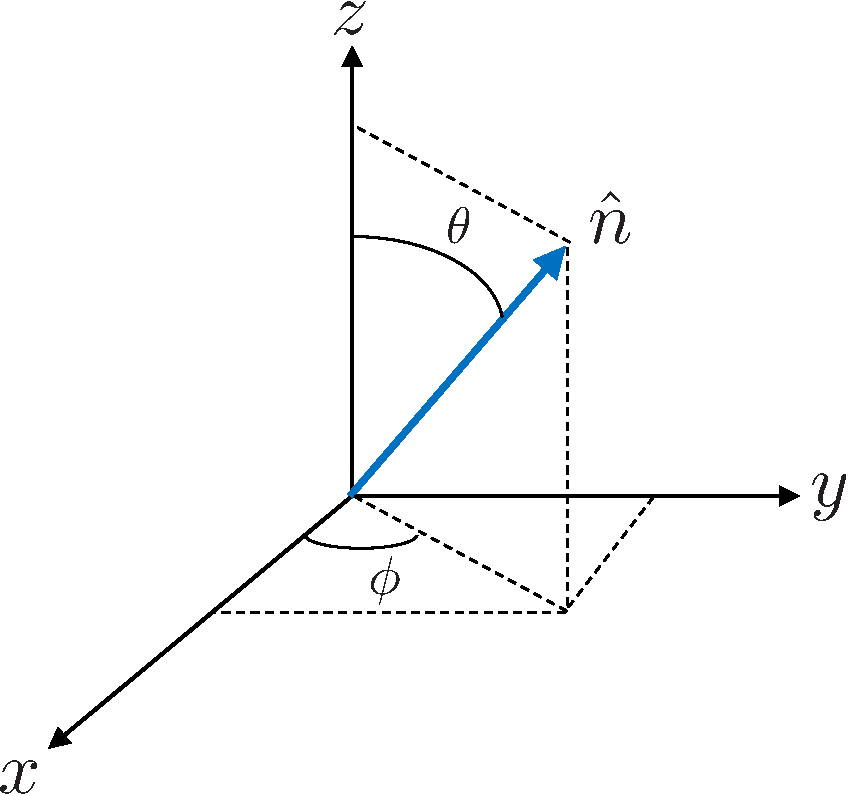
\includegraphics[width=0.48\textwidth]{Figures/rotation0-crop.pdf}\\[1ex]
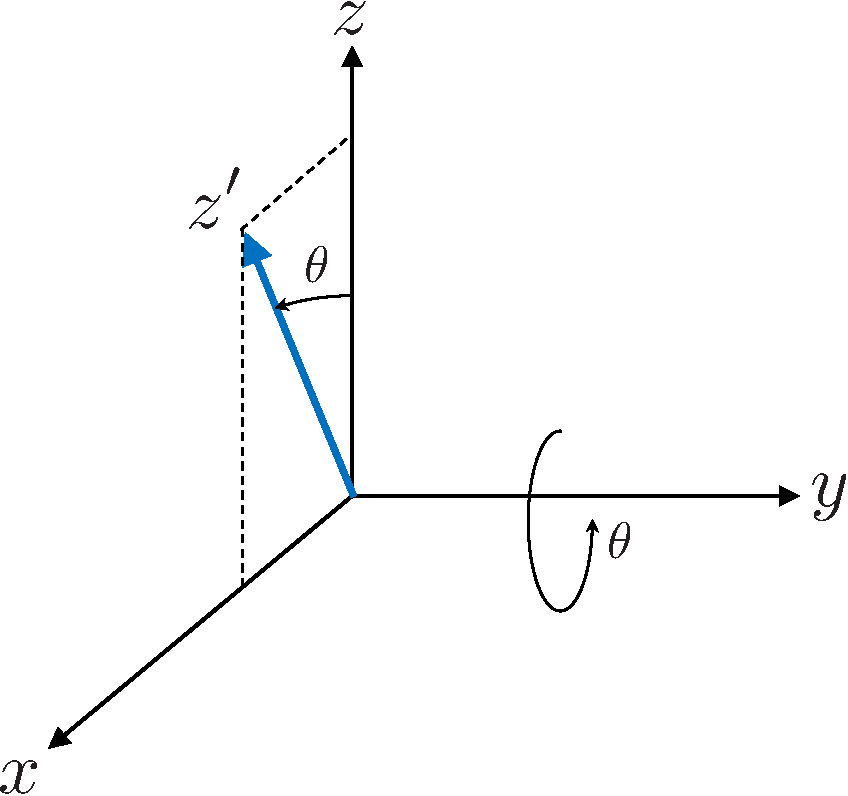
\includegraphics[width=0.48\textwidth]{Figures/rotation1-crop.pdf}
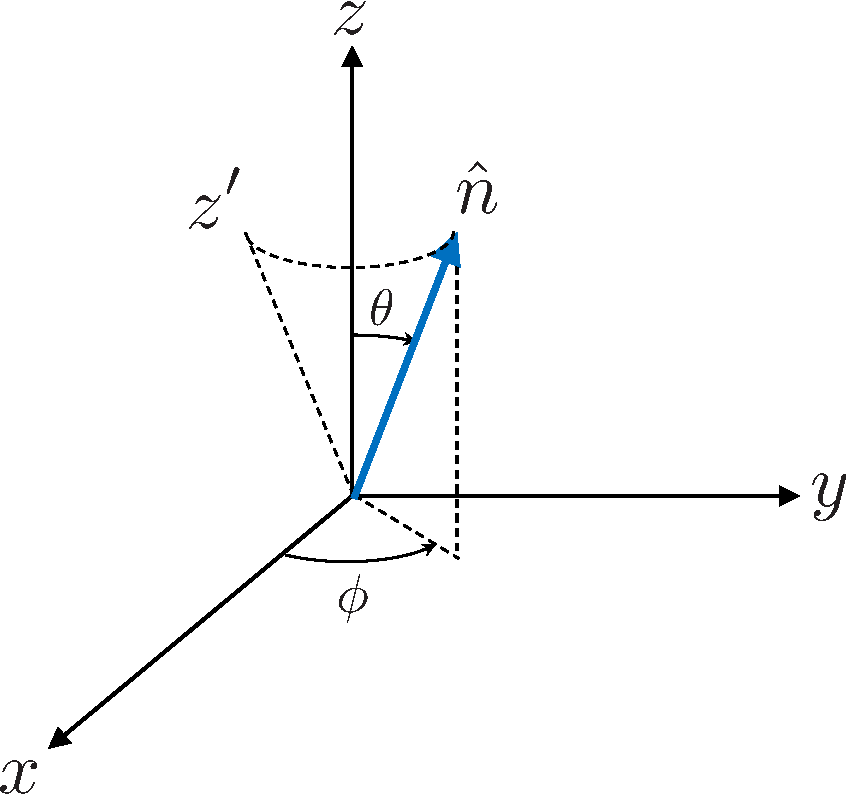
\includegraphics[width=0.48\textwidth]{Figures/rotation2-crop.pdf}
\end{center}

One could have rotated first by an angle \(\psi\) about \(z\)
\(\Rightarrow\) this extra rotation would not change the final
axis $\hat{n}$:
\be
R(\theta, \phi) \rightarrow R(\theta, \phi, \psi)=R(\theta, \phi) e^{-i / \hbar \psi \hat{J}_{z}}
\ee
The net effect would be an extra phase in $\ket{jm} \to \ket{jm}_R$:
\[
\ket{jm}_{R(\theta, \phi, \psi)} = 
\hat{U}[R(\theta, \phi)] e^{-i / \hbar \psi \hat{J}_{z}} \ket{jm} = 
e^{-im\psi} \ket{jm}_{R(\theta, \phi)}
\]
The rotation here corresponds to Euler angles: \(\alpha=\phi, \beta=\theta, \gamma=\psi=0\)

%%% 13 OKAY

The unitary operator \(\hat{U}[R(\theta, \phi)]\) is given by
\be
\hat{U}[R(\theta, \phi)]=e^{-i/\hbar \phi \hat{J}_{z}} e^{-i/\hbar \theta \hat{J}_{y}}
\ee
and its matrix elements in the basis $\ket{jm}$ are given by
\be
\begin{aligned}
\left\langle j m^{\prime}|\hat{U}[R(\theta, \phi)]| j m\right\rangle 
& \equiv D_{m^{\prime} m}^{(j)}(\theta, \phi) \\ 
&=\left\langle j m^{\prime}\left|e^{-i/\hbar \phi \hat{J}_{z}} e^{-i/\hbar \theta \hat{J}_{y}}\right| j m\right\rangle \\ 
&=e^{-i m^{\prime} \phi}\left\langle j m^{\prime}\left|e^{-i \theta \hat{J}_{y}}\right| j m\right\rangle \\
&=e^{-i m^{\prime} \phi} d_{m^{\prime} m}^{(j)}(\theta)
\end{aligned}
\ee
where $d_{m^{\prime} m}^{(j)}(\theta)$ are the matrix elements of $\hat{U}[R_y(\theta)]$:
\be
d_{m^{\prime} m}^{(j)}(\theta) =
\bra{jm^\prime}
e^{-i/\hbar\theta\hat{J}_y}
\ket{jm}
\ee

From the group property of the rotation, that is from
the group property of the $D^{(j)}$ matrix one obtains:
\be
d_{m^{\prime} m}^{(j)}(\theta_1+\theta_2) =
\sum_{m^{\prime\prime}}
d_{m^{\prime} m^{\prime\prime}}^{(j)}(\theta_1)
d_{m^{\prime\prime} m}         ^{(j)}(\theta_2)
\ee
In addition, from the group property
\be
\hat{U}^\dagger[R] = \hat{U}^{-1}[R] = \hat{U}[-R] 
\ee
one has (\emph{Exercise})
\be
[d_{m^{\prime} m}^{(j)}(\theta)]^\dagger =
d_{m^{\prime} m}^{(j)}(-\theta)
\ee
In addition (\emph{Exercise}):
\be
d_{m^{\prime} m}^{(j)}(\theta) = (-1)^{m-m^\prime}
d_{-m^{\prime},-m}^{(j)}(\theta)
\ee

%%% 14 OKAY

Coming back to the $\pm$ sign in \(\hat{U}\left(g_{2}\right) \hat{U}\left(g_{1}\right)=\pm \hat{U}\left(g_{2} g_{1}\right)\)
-- let us consider two sucessive rotations about the
\(Oz\) axis by angles \(\theta_{1}\) and \(\theta_{2}\) such that
\be
\theta_{1}+\theta_{2}=\theta+2 \pi n, 
\quad 0 \leqslant \theta \leqslant 2 \pi, \text { integer } n>0
\ee
then
\begin{gather}
\begin{gathered}
\bra{jm^\prime}\hat{U}[R(\theta+2\pi n)]\ket{jm}= 
\bra{jm^\prime}
e^{-i/\hbar\theta\hat{J}_z}
e^{-i/\hbar(2\pi n)\hat{J}_z}
\ket{jm}\\
=\delta_{m^{\prime} m} e^{-i \theta} e^{-i(2 \pi n) m}=\delta_{m^{\prime} m} e^{-i \theta}\left(e^{-i 2 \pi m}\right)^{n}
\end{gathered}\\
=\delta_{m^{\prime} m} e^{-i \theta} \times
\begin{cases}
+1,       & \text{ $m$ integer} \Rightarrow \text{ $j$ integer}\\
(-1)^{n}, & \text{ $m$ 1/2-integer} \Rightarrow \text{ $j$ 1/2-integer}\\
\end{cases}
\label{eq:g96}
\end{gather}
$Oz$ axis is arbitrary; therefore, the result \eqref{eq:g96}
is valid for an arbitrary direction $\hat{n}$, that is:
\be
e^{-i/\hbar \theta \hat{n}\cdot\hat{\vec{J}}}
\left(e^{-i/\hbar 2\pi \hat{n}\cdot\hat{\vec{J}}}\right)^n
=
e^{-i/\hbar \theta \hat{n}\cdot\hat{\vec{J}}} \times
\begin{cases}
+1,       & \text{ $j$ integer}\\
(-1)^{n}, & \text{ $j$ 1/2-integer}\\
\end{cases}
\ee
hence
\be
\hat{U}[R_2]\hat{U}[R_1] =
\begin{cases}
+\hat{U}[R_2R_1]\\
\pm\hat{U}[R_2R_1]
\end{cases}
\ee
\emph{Conclusion:} to any rotation there correspond \emph{two}
rotation operators of opposite sign for \(1 / 2\)-integer \(j\)
and only one for \(j\) integer.

%%% 15 OKAY
\clearpage

\emph{Example:} $j=1/2$
\[
d^{1 / 2}(\theta)=e^{-i \theta / 2 \sigma_{y}}=\cos \theta / 2-i \sin \theta / 2
\]
and its representation in the basis
$\ket{jm} = \ket{1/2,\pm1/2} \to \{\ket{+},\ket{-}\}$
\be
d^{1/2}(\theta) =
\begin{pmatrix}
\cos \theta/2 & -\sin \theta/2 \\
\sin \theta/2 &  \cos \theta/2
\end{pmatrix}
\ee
leads to
\be
D^{1/2}(\theta,\phi) =
\begin{pmatrix}
e^{-i\phi/2}\cos \theta/2 & -e^{-i\phi/2}\sin \theta/2 \\
e^{i\phi/2}\sin \theta/2  &  e^{i\phi/2}\cos \theta/2
\end{pmatrix}
\ee
\emph{Exercise:} show that this representation is \emph{irreducible}.

\emph{Summing up:}
\begin{itemize}
\item consider a rotation by $\theta=2\pi$ about $\hat{n}=\hat{z}(\phi=0)$
\be
D^{(1 / 2)}(0,0)=I, \quad D^{(1 / 2)}(2 \pi, 0)=-I
\ee
\item these matrices provide a double-valued representation
of the rotation group, \(SO(3)\): \(\theta=0\) and \(\theta=2 \pi\) correspond
to the same element of \(SO(3)\), the identity.
\begin{gather}
R(\theta)
\Rightarrow
\begin{pmatrix}
V_x^\prime\\V_y^\prime\\V_z^\prime
\end{pmatrix}
=
\begin{pmatrix}
\cos\theta & -\sin\theta & 0\\
\sin\theta & \cos\theta & 0\\
0 & 0 & 1
\end{pmatrix}
\begin{pmatrix}
V_x\\V_y\\V_z
\end{pmatrix}
\\\nonumber\\
%%% 16 OKAY
\to R(0) = R(2\pi) = I
\end{gather}
\item however the \(D^{(1 / 2)}(\theta, \phi)\) form a \emph{single-valued}
representation of another group, \(SU(2)\), which
acts on the two-dimensional complex vector space
of complex 2-vectors, leaving invariant the scalar
product of such vectors:
\be
D^{(1 / 2)}(\theta, \phi)
\begin{pmatrix}u_{1} \\ u_{2}\end{pmatrix}=
\begin{pmatrix}u_{1}^{\prime} \\ u_{2}^{\prime}\end{pmatrix},
\left|u_{1}^{\prime}\right|^{2}+\left|u_{2}^{\prime}\right|^{2}=\left|u_{1}\right|^{2}+\left|u_{2}\right|^{2}
\ee
%
\be
\begin{aligned}
\begin{pmatrix}
u_2^\prime\\u_2^\prime
\end{pmatrix}
=
\begin{pmatrix}
e^{-i\phi/2}\cos \theta/2 & -e^{-i\phi/2}\sin \theta/2 \\
e^{i\phi/2}\sin \theta/2  &  e^{i\phi/2}\cos \theta/2
\end{pmatrix}
\begin{pmatrix}
u_1\\u_2
\end{pmatrix}\\
\begin{pmatrix}
e^{-i\phi/2}\cos \theta/2 u_1 - e^{-i\phi/2}\sin \theta/2 u_2\\
e^{i\phi/2}\sin \theta/2  u_1 + e^{i\phi/2}\cos \theta/2 u_2
\end{pmatrix}
\end{aligned}
\ee
So
\be
\begin{aligned}
\left|u_{1}^{\prime}\right|^{2}+\left|u_{2}^{\prime}\right|^{2} 
&=\cos ^{2} \theta / 2\left|u_{1}\right|^{2}-\cancel{\left(u_{1}^{*} u_{2}+u_{2}^{*} u_{1}\right)} \cos \theta / 2 \sin \theta / 2 \\ 
&+\sin ^{2} \theta / 2\left|u_{2}\right|^{2}+\sin ^{2} \theta / 2\left|u_{1}\right|^{2} \\ 
&+\cancel{\left(u_{1}^{*} u_{2}+u_{2}^{*} u_{1}\right)} \sin \theta / 2 \cos \theta / 2\\
&=\left(\cos ^{2} \theta / 2+\sin ^{2} \theta /2\right)\left(\left|u_{1}\right|^{2}+\left|u_{2}\right|^{2}\right)=\left|u_{1}\right|^{2}+\left|u_{2}\right|^{2}
\end{aligned}
\ee
So for $j = 1/2$
\be
\begin{gathered}
\begin{pmatrix}u_1\\u_2\end{pmatrix} \to \ket{1/2,m} = 
D^{1/2}_{m^\prime m}(\theta,\phi) \ket{1/2,m^\prime}\\
\ket{1/2,m} \to e^{-i/2\hbar\hat{n}\cdot\vec{\sigma}} \ket{1/2,m}
\end{gathered}
\ee
%%% 17 OKAY
\item the representation is single-valued because
\(\theta=0\) and \(\theta=2 \pi\) represent \emph{two} distinct
elements of \(SU(2)\).
\end{itemize}

This group is important for several reasons; in
the present context it is important because all
the higher-dimensional representations \(D^{(j)}\) can
be constructed from \(D^{(1 / 2)}\) by coupling angular
momentum:
\(\nicefrac{1}{2}\,\oplus\,\nicefrac{1}{2} \rightarrow 1\), 
\(1\,\oplus\,\nicefrac{1}{2}\rightarrow\nicefrac{3}{2}\), 
\(\nicefrac{3}{2}\,\oplus\,\nicefrac{1}{2}\rightarrow 2\), \ldots













\end{document}
